\chapter{Phenotyping and re-sequencing a high fitness line from a modified mutation accumulation experiment} 
 \vspace{2cm}
 
\section{Abstract}
Our understanding of adaptive evolution relies on determining the frequency, magnitude of fitness effect and genomic architecture of beneficial mutations. However, theoretical work and empirical observations find that mutations with positive effects on fitness are rare. Here, I used the opportunity of a single serendipitous observation of high competitive mating success in a \textit{Drosophila serrata} mutation accumulation (MA) subline to further investigate putative casual loci. Prior to detection, MA lines were subdivided and maintained at two population size treatments, small ($N = 24$) and large ($N = 288$), for seven generations; altering the threshold that segregating mutations were visible to selection ($s = 1/2N_e$). I used whole-genome sequencing on pooled flies sampled separately for each subline, in each sequential generation, to identify patterns of genomic sweeps. I observed patterns of increased selection against multiple deleterious variants with small effect sizes ($\sim 0.003 < s < 0.029$), but I was unsuccessful in confirming my \textit{a priori} expectation of detecting a single large-effect causal locus. I further propose a series of recommendations for data analysis. Considering these recommendations, my findings suggest that my analytical approach has the potential for detecting adaptive mutations undergoing genetics sweeps whilst simultaneously inferring the distribution of fitness effects. \par

\newpage

\section{Introduction} 
Mutations with positive effects on fitness are essential for adaptive evolution yet appear to comprise a small fraction of all spontaneous mutations \citep{Fish30, Simm77, Houl96, Lync99, Keig03, Eyre07, Hall09}. Theoretical justification for the rareness of beneficial mutations comes from Fisher’s geometric model of adaption \citep[FGM,][]{Fish30} which posits that, in a multidimensional fitness landscape, it is more likely for a mutation to move the individual further from, rather than nearer to, the local fitness peak. Fisher further demonstrated that mutations of infinitesimally small effect had the highest probability of being favourable, whereas large effect mutations are more likely to be harmful, and thus unimportant for adaptation in natural populations \citep{Fish30}. Theoretical work on beneficial mutations has extended into considering visibility of beneficial alleles to selection \citep[intermediate effect mutations are more likely to overcome stochastic process at initial frequencies,][]{Kimu83}, and the context of the genetic background (which will determine the distance from the local fitness optima) in which that mutation arises \citep{Orr98}. However, the general principle that advantageous mutations are rare still holds \citep{Houl96, Lync99, Hall09}.\par

Contrary to the bulk of the empirical evidence, several studies have reported naturally arising beneficial mutations in mutation accumulation studies (MA). For the microbial species \textit{Saccharomyces cerevisiae} and \textit{Dictyostelium discoideum}, 6 – 40\% of mutations \citep{Wloc01, Zeyl01, Jose04, Hall13amoeba} increased fitness. However, this inference of up to 40\% beneficial mutations may be inflated due to the growth periods between colony picking (i.e., increasing population size), which may allow selection to enrich for beneficial mutations \citep{Jose04, Wahl22}. An early study of a single \textit{Arabidopsis thaliana} line also suggested an equal frequency of beneficial and deleterious mutations \citep{Shaw02}. However, \citet{Shaw02}’s conclusions were challenged by \citet{Keig03} on three grounds: 1) there were insufficient generations (17) to detect a significant mean fitness decline; 2) the focal traits might be under stabilising selection and therefore not genuine fitness components, and; 3) alternative models for the distribution of mutational effect were not considered. Nonetheless, several further studies of \textit{Arabidopsis} lines have also reported beneficial mutations to be common \citep{Chan03, Kava05, Rutt10, Role16}. \par

The frequency at which new beneficial alleles arise is not enough, on its own, to predict the rate of adaptive change; the magnitude of effect that a new mutant allele has on fitness must simultaneously be considered. Mutations vary widely in their effect on fitness \citep{Eyre07, Wals18c10} where mutations with weak effects \citep[$s < 1/2N_e$, where $s$ is the selection coefficient and $N_e$ is the effective population size][]{Wrig31, Kimu83} evolve under drift, while the fate of mutations with larger effects on fitness will be determined by selection. While Fisher’s geometric model envisions adaptation as a result of many loci of infinitesimal effect, \citet{Kimu83} highlights that beneficial mutations of intermediate to large effect had a greater probability of overcoming drift. Accordingly, extreme value theory has described this distribution of effect as exponential \citep{Gill84, Orr03}, where observation from several studies conform to many beneficial mutations of small effect and few of large effect \citep{Imho01, Kass06, Burc07, Bata11}. Evidence of very rapid fitness recovery of low-fitness populations when selection is allowed to operate suggests sufficient number and effect size of beneficial mutations arise to recover (and maintain) fitness \citep{Burc99, Este03, Este11, Szam14}. For example, in \textit{Caenorhabditis elegans}, \citet{Este03} observed that low-fitness MA genomes display quick ancestral fitness recovery when selection is re-introduced ($< 10$ generations).\par

Whole genome sequencing (WGS) of populations evolving via accumulation of spontaneous mutations has improved estimates of the genomic mutation rate and the nature of new mutations \citep[reviewed by][]{Katj19}. Although mutations with known fitness effects in specific contexts (e.g., antibiotic resistance) have been characterised, in general, genome sequencing has relatively rarely been used to characterise new mutations with known fitness effects. Applying whole genome sequence analyses on three fitness-recovered \textit{C. elegans} lines (Estes), \citet{Denv10} uncovered patterns of rapid selective sweeps (10-20 generations) for between 7 and 12 novel mutations. Genomic studies of adaptation in genetically diverse, outbred, populations suggest that a model of a single unconditionally advantageous allele sweeping through a population is exceptional, and that it is more typical that multiple alleles of small effect contribution to adaptive fitness \citep{Prit10, Barg19}. It, therefore, remains an open question whether the distribution of effect sizes of novel beneficial mutations differs from the effect sizes of variants that persist in standing genetic variation. \par

With the present study, I take advantage of a serendipitous observation of a high fitness genotype to investigate the characteristics of beneficial mutations and evolution of increased fitness. A panel of 42 \textit{Drosophila serrata} lines that had previously accumulated mutations for 20 generations was subdivided into two different population size treatments (described in detail in Chapter 2). Nine generations after line subdivision, male competitive fitness was measured in all 84 sublines (see Methods). Extremely high fitness, 5.5 SD above the mean fitness, was observed in the large population size copy of one MA line, L9 (see Results). Relative to reported average declines in fitness in MA lines \citep[0.36\% per generation,][]{Hall09}, the magnitude of the phenotypic effect observed in the \textit{D.~serrata} line may reflect a large effect beneficial mutation, depending on when in the nine generations of evolution it arose. Taking advantage of a complete time-series of genomic samples from the two copies of this subdivided MA line (one with high fitness and one with average fitness), I investigate the genomic change that facilitated the elevated fitness, and the temporal trajectory of the genetic change. I first confirm that the elevated fitness was not due to immigration from a high-fitness outbred population. I then sought to identify loci with divergent allele frequencies between the high and average fitness lines that shared a very recent ($<10$ generations) common ancestor.\par


\section{Methods}
\subsection{Competitive fitness for \textit{Drosophila serrata} experimental populations}
\subsubsection{Generation and maintenance of experimental populations}

The history of the experimental populations reported here is outlined in Chapter 2. Briefly, 200 mutation accumulation (MA) lines were established from a single \textit{D. serrata} Reference Genome Panel (DsRGP) line \citep{Redd18} and maintained via sibling-mating. Genome-wide heterozygosity for this DsRGP line was low (0.3\%). This degree of residual heterozygosity in inbred lines used as MA ancestors is likely common but seldom quantified. After 20 generations of brother-sister matings (i.e., the mutation accumulation phase), the residual heterozygosity of 0.03\% should decrease, where 1/2N decrease in heterozygosity per generation \citep{Fran02} predicts an expected residual heterozygosity of $\sim 1$ in 1,000,000 sites. From these MA lines, 42 lines were randomly chosen and expanded over three generations to establish two sublines in population size treatments. For each of the 42 lines, a small (S: $N = 24$ flies per line) and large (L: $N = 288$) population size treatment was established. For both treatments, flies were maintained synchronously as 12 males and 12 females per vial to ensure flies experienced a similar larval environment, with the L lines maintained in 12 vials of 24 flies each. \par

We used the average estimate of single nucleotide mutation rate for \textit{D. melanogaster} as $5.02\times10^{-9}$ per site per generation \citep{Katj19} and scaling this to the 198 M$bp$ \textit{D.~serrata} female genome size \citep{Alle17B}[($5.02\times10^{-9}/2$) $\times$ $2N \times$ generations $\times$ 198 M$bp$] where 2$N$ reflects the number of diploids per line), to predict the number of mutations that would arise. After expansion and application of population treatments, I would expect 262 and 2370 introduced mutations in the small and large populations, respectively; calculated by substituting the effective population size for laboratory raised \textit{Drosophila melanogaster}, $N_e = 0.7N$ \citep{Crow55}, and assuming neutrality of all mutations. Substituting the per-site residual heterozygosity expectation after inbreeding into this formula, we would expect an additional $\sim792$ segregating ancestral variants.  This elevated number of mutations segregating between sublines sharing a single ancestor is still well below that expected for outbred populations but nonetheless raises the challenge of discerning the pattern of selection whether a strong, soft or polygenic sweep, against a noisy molecular background \citep{Wals18c9}.\par

\subsubsection{Fitness assays} 
I conducted a competitive fitness assay after five generations of maintenance at the two different population sizes. Two replicate rearing vials per MA line per treatment were established by three males and three females per vial in the generation prior to the fitness assay. Four competitive fitness assays were initiated per replicate rearing vial, per treatment (2), per line (42), giving a maximum possible 672 fitness assay vials. Competitive fitness assays consisted of two focal males (from the same replicate rearing vial), two competitor orange-eyed males and two orange-eyed females, where the orange-eye phenotype is recessive to the wildtype red-eye, allowing paternity to be readily inferred \citep{Alle17}. The orange eye \textit{D. serrata} competitor stock had been inbred repeatedly and maintained at a moderate population size (150 founders each generation) for several generations. Fitness assay flies were left to mate and lay on a standard 10mL yeast medium \citep{Rund05}, with a small amount of live yeast, for four days before adults were cleared. Total emergence was collected from each vial, and the number of red and orange-eyed offspring was counted. Competitive fitness was calculated as \citep{Alle17}: 
$log_{10}(\frac{1+Red\ eye}{1+Orange\ eye})$, where I added one to each count to prevent observed counts of zero being undefined. This data was normally distributed when placed on a log scale. A total of 14 vials had zero offspring and were excluded from analyses. Ten observations were 3.0 to 3.5 standard deviations (SD) above the mean; I consider outliers in more detail in the Results.\par

\subsubsection{Analyses of variation in fitness}
The population size treatments imposed ensured that mutations differ by approximately an order of magnitude in their visibility to selection (mutations evolve under drift when $s < 1/2N_e$). I tested whether this difference in the opportunity for selection had caused evolution of mean fitness or of the genetic variance for fitness. To do this, I fit a mixed model in which I treated fitness as a separate trait in each treatment, an approach commonly used for estimating the genetic correlation for a trait expressed in different environments \citep{Falc96} or different sexes \citep{Alle17}. I fit the following mixed model using the MIXED procedure in SAS v9.4 (SAS Institute Inc., Cary, NC.):

\begin{equation}
\label{eqn:FitlogOR}
y_{ijkm}=\mu + Treat_i + Line_j + Vial_{k(ij)} + \varepsilon_{ijkm}
\end{equation}

\noindent where $y$ was the vector of competitive fitness scores for each replicate vial per MA line per treatment, $\mu$ was the population intercept, and treatment (Treat) was fit as a fixed effect. At the among-line level (Line) I modelled a covariance structure that allowed me to estimate the among-line variance within each treatment, and the correlation between treatments. Replicate rearing vial (Vial) and individual fitness assays ($\varepsilon$), where the vials and individuals differed between the population size treatments, were modelled as diagonal matrices, with treatment-specific variances, but no among-treatment covariance. \par

First, I determined whether mean fitness differed between treatments, fitting model (\ref{eqn:FitlogOR}) using maximum likelihood, and assessing the ANOVA output. Next, I fit model (\ref{eqn:FitlogOR}) using restricted maximum-likelihood to test whether there was statistical support for among-line variance for competitive fitness within each treatment using Likelihood Ratio Tests, LRTs (1 d.f.), to compare a model in which the variance was estimated to a model in which the treatment’s among-line variance was constrained to zero (implemented using the PARMs option). Next, LRTs comparing the estimated and constrained models (again implemented using the PARMs option) were used to test the hypotheses that the between treatment genetic correlation was not significantly different from one or from zero. Lastly, I also used LRT to determine whether a single estimate of variance for both treatments or treatment-specific variance estimates (fit using autoregressive covariance structures with homogenous or heterogeneous variances, respectively) better fit the data. \par

\subsection{Temporal sequencing and resequencing of a single high fitness line}
\subsubsection{DNA extraction and genome assembly}
For each line, 40 females were collected each generation (beginning in the second generation during line expansion), resulting in seven generations of samples, which were all stored at $-80\degree$C. I sequenced the pooled genomes of these 40 female flies collected for Line 9 in the S and L treatments (14 pools in total). Sampling females ensures a balanced sample size across both the autosomes and the X chromosome. For each pool, tissue was homogenised and DNA was extracted using the Gentra Puregene Core Kit A (Qiagen). Extracted DNA was then cleaned of impurities using PCRdx magnetic beads (Aline Biosciences), following New England BioLabs protocols developed for AMPure beads. Samples were then sent to Novogene for library construction (Plant and Animal Whole Genome resequencing library) and genome sequencing. One hundred and fifty base pair (bp) paired-end sequences were constructed and sequenced using an Illumina NovaSeq PE150 platform. I assessed the raw fastq sequence quality using FastQC v.0.11.8 \citep{Andr12}, where for each of the twenty-eight fastq files (14 pools, replicated twice), all 150bp positions had mean Phred quality scores that exceeded 28 (approximately a 99.9\% base call accuracy). The raw sequences were mapped to the \textit{D. serrata} reference genome \citep{Alle17B}, annotated by \citet{Redd18}, using BWA-mem v.0.7.13 \citep{Li09bwa}.\par 

Post alignment, the SAMtools v.1.3 \citep{Li09samtools} application was used to convert SAM files to BAM files where reads were filtered for a minimum mapping quality of 20. Quality control for contiguous sequence alignment against the reference genome was performed using the bamqc and multi-bamqc functions from the Qualimap 2.2.1 application \citep{Garc12Qualimap, Okon16}. The mean coverage for each of my 14 samples ranged from 48.5 to 86.7x (Table \ref{tab:DNAsuppQualimap}). BAM files were further filtered for duplicate reads with Picard MarkDuplicates and corrected for overlapping read pairs (BamUtil version 1.04.14). To improve subsequent genomic analyses, I used a subset of only the seven longest localised scaffolds which represented the majority of all major chromosome arms (2L, 2R, 3L, 3R and X) and accounted for 79.73\% of the total assembly (total assembly: 198,341,263 bp). Lastly, I applied pool-specific coverage limits across all loci, setting the thresholds as the median read depth $\pm$ twice the interquartile range (IQR) (Figure \ref{fig:DNAsuppDepthHist}). The upper threshold excludes potential paralogue loci and the lower threshold excludes poor read depth. Low read depth results in allele frequency bias where read depth should ideally equal the number of chromosomes within the pool 
\citep[here $\sim80$,][]{Futs10,Kola11,Lync14}, however setting a global coverage minimum would have preclude me from analysing pools with poorer coverage.\par

\subsubsection{Nucleotide diversity}
The low fitness of inbred lines, including MA lines, makes them vulnerable to invasion by high fitness, outbred, genotypes; such contamination has been previously observed in a \textit{D. melanogaster} MA experiment \citep[as described in ][]{Houl94}. Population genomic variation was assessed independently for each of the pools, where large deviations in nucleotide diversity estimates across generations could be indicative of an invasion event. For a completely replaced pool, low within-pool diversity is expected but regions of the genome would be highly diverged when contrasted against other pools. Whereas I would expect high within-pool diversity to occur in the generations immediately after a high-fitness individual immigrant, due to newly introduced alleles. Analyses were implemented using a pipeline from POPOOLATION v.1.2.2 \citep{Kofl11}, a program that accounts for pooled sequencing by incorporating the pool-size, coverage thresholds, and lack of discrete genotypes. I estimated both Tajima’s nucleotide diversity \citep[$\pi$,][]{Taji83}, which quantifies nucleotide polymorphisms across loci, and Tajima’s D, a test that contrasts the number of segregating sites against intermediate-frequency sites \citep[for a population at mutation-drift equilibrium, these two estimates should be approximate,][]{Taji89}. First, I converted the BAM files to the required mpileup format using SAMtools, then small insertions and deletions (indels) were identified using the POPOOLATION identify-genomic-indel-regions.pl script and removed using filter-pileup-by-gtf.pl. As estimates of diversity within populations are sensitive to sequencing error, poorly mapped reads and insufficient coverage \citep{Kofl11}, I subsampled each mpileup file to a uniform coverage using the pool-specific limits (Figure \ref{fig:DNAsuppDepthHist}) implemented with the subsample-pileup.pl script. The resulting files were then used to simultaneously calculate $\pi$ and Tajima’s D, implemented with the Variance-sliding.pl script, for 50 kb non-overlapping windows and a recommended minimum minor allele count of two \citep{Kofl11}. I used R (v. 4.0.2) to preform Kruskal-Wallis rank sum tests to determine if $\pi$ and Tajima’s D differed among pools. For Tajima’s D estimates, I rejected the null hypothesis (see Results) where I applied further post-hoc pairwise tests for treatment differences across and within generations, using the Benjamini-Hochberg method \citep{Benj95} to correct for multiple hypothesis testing (for the seven generations), using a conservative 5\% false discovery rate (FDR). \par

\subsubsection{Variant Calling and loci filtering}
Despite POPOOLATION (above) using SNPs to estimate population genetic parameters, this software was not conceived as a SNP caller \citep{Rain12} and additionally excludes detection of small indels; mutations that are more likely to have a nonsynonymous effect on fitness \citep{Sung16}. Here I identify variable genomic regions and apply quality filtering to establish a dataset for investigating putative causal loci for the observed high fitness (below). Variant calling was performed on each pool individually using FreeBayes \citep{Garr12}, where I implemented parallelised processing on separate regions of the genome for each sample (\textit{freebayes-parallel}; parameter settings as per Table \ref{tab:DNAsuppFreeBayParms}). The default variant calling format (VCF) reports only positions that are variable relative to the reference genome, presenting a threefold problem for identifying variable loci within my experiment. First, missing data within a pool was confounded with invariant homozygous reference loci, therefore I included the ‘report monomorphic’ (homozygous reference) option within Freebayes to overcome this. Second, within each pool, loci that differed from the reference, but were fixed within the pool, were reported as variable; these loci were only identified once data for all fourteen pools was concatenated (described below). Lastly, the raw VCF files report loci that were biallelic for two alleles that were not identical to the reference allele as triallelic. To overcome this, I used Vcflib tools \citep{Garr16} to separate multiallelic genotypes for post-processing in R. Also, using Vcflib tools, haplotypes were partitioned into single nucleotide variants and indels, where I considered all mismatches, insertions, and deletions as candidate causal mutations. \par

All fourteen VCF files were imported into R and merged using the data.table package \citep{Dowl20}. To further reduce sequencing error influencing results, particularly mis-identified multiallelic loci, I removed alleles that were only represented in a single pool (singletons) (this step could potentially exclude the causal allele if it was present only in the last generation of the large population, but I explain below that I had little confidence in the sampling of this pool). I also ensured that all alleles were covered by at least two reads within a pool (unless loci had been flagged as homozygous for the reference loci, in which case a read depth of zero for an alternate allele was permitted) \citep{Kofl11}. Invariant loci were identified across all fourteen pools and removed (upwardly inflated due to monomorphic sites and misidentified biallelic loci). I retained loci with missing data only in the Large treatment in the seventh generation, as this pool had the poorest read depth (Figure \ref{fig:DNAsuppDepthHist}; Table \ref{tab:DNAsuppQualimap}). These steps resulted in 232,124 biallelic (98.5\%) and 3,464 triallelic (1.5\%) variant loci. I kept only the biallelic loci for further analyses as triallelic loci are extreme rarities at nucleotide sites \citep{Burk10,Lync14}, and I expected many of these to be misreads.\par

\subsubsection{Determining mutant alleles causing fitness divergence}
Here I aim to identify the genetic changes responsible for the observed high fitness of the Line 9 large population size treatment. This phenotype occurred at high frequency (all eight replicate vials in the fitness assay) suggesting that the causal allele(s) are also likely to be segregating at high frequency by the final generation of my experiment, and that I may detect increasing frequency of these allele(s) across the earlier generations. As I did not observe high fitness in the small population size treatment, the high fitness allele is predicted to have arisen after the MA line was divided into these two treatments. It is important to note that allowing loci to have alternative allele counts of zero within certain treatments precluded me from imputing allele frequencies using applications such as POOLNE\_ESTIM \citep{Gaut13}, PoPoolation \citep{Kofl11} or poolFreqDiff \citep{Wibe17}. Instead, based on these broad expectations, I further refined the set of candidate loci analysed, and developed analytical approaches to reflect the unusual structure of my data. \par

The S treatment in the first generation of sampling was considered the best representative of the MA ancestor, and therefore, the allele with the highest frequency in this pool was designated the focal (ancestral, major) allele, while the alternate (low frequency, minor) allele was designated as the derived allele. For some loci, in generation 1 of the S treatment, alternate alleles were observed at equal frequencies ($p = q = 0.5$). For these loci, I used the L treatment in generation 1 as the reference; if a clear major versus minor allele could still not be determined, I considered the second generation in the S treatment, and if that information was similarly uninformative, I considered the L treatment. I then identified loci that were poorly sampled based on repeated patterns of apparent gain and loss of the alternative allele within either the L or S pools. This was done by applying a present/absent/present rule across sliding windows of three or more consecutively sampled generations (ignoring missing data) and excluded loci with alleles that, after the initial generation, were sporadically unsampled (zero reads). I also considered loci poorly sampled if I observed extreme allele frequency changes ($|p| >0.6$) that lacked consistent divergence (e.g. not continually increasing or decreasing across time) and excluded these loci (Figure \ref{fig:DNAsuppBouncyP}). I also redefined the mutation type with regards to the focal allele (VCF uses the reference genome allele), categorising mutations as either SNPs or indels (where I categorised single nucleotide deletions as SNPs rather than as indels). Lastly, I excluded any locus with a maximum (across all 14 pools) minor allele frequency, $q$, $< 0.05$ (Figure \ref{fig:FitmxMAF}), given that I expected causal loci to be at high frequency in at least some pools to account for the fitness variation observed. These further quality control steps resulted in 98,189 biallelic loci (84,401 SNPs; 13,788 indels) that were retained for analysis.\par

I first consider four general scenarios that might have led to the observed fitness divergence, two in which the mutation arose after line subdivision, and two in which it arose in the MA phase (but did not fix prior to establishment of S and L sublines). First, the high fitness of L could be due to mutation(s) that arose after line subdivision, resulting in a pattern where the major allele was fixed within the S treatment and the minor (derived) allele was at relatively high frequency within the terminal generation(s) of the L treatment (Figure \ref{fig:FitScenario}, top left). Second, the high fitness allele may have been fixed in the MA period of the experiment (i.e., been the major allele), followed by a secondary mutation (reversion or novel deleterious mutant) in S subline, which increased in frequency under drift (Figure \ref{fig:FitScenario}, bottom left). Third, the stronger selection in L may have driven the high fitness mutation toward fixation (and the ancestral, major, allele to loss: Figure \ref{fig:FitScenario}, top right). Fourth, the stronger drift in S could have caused the high fitness mutation to be lost (and the ancestral allele to be fixed: Figure \ref{fig:FitScenario}, bottom right). Notably, while the alternative alleles at the causal locus (loci) might be fixed in S versus L, it is more likely that alleles are still segregating in at least one of the sublines.\par

To identify putative causal loci, I used a two-step approach: first, I identified outlier loci for the sixth and seventh (terminal) generations using two different measures of allelic difference between the S and L subline; then, I determined if these outlier loci were consistently diverging over time, using my sequential repeated-measures experimental design. It is worth noting that my approach is an enrichment method and only suggests potential targets of the genome that might harbour a beneficial mutation. \par

$F_{ST}$ is an appropriate measure to determine selection candidates, provided alleles are at intermediate values \citep[MAF $\geq$ 0.05,][]{Bern19}; loci with minor allele frequencies $< 0.05$ were excluded from this analysis. I investigated outlier loci within the one-tailed ($95^{th}$ percentile) pairwise $F_{ST}$ distribution for the sixth and seventh (terminal) generations, investigating SNPs and indels separately. Generally, when searching for genes underlying adaptive traits, 5–10\% of loci are reported as outliers \citep{Stin08, Nosi09}; however, due to the magnitude of the observed fitness, I only considered loci falling within a modest 5\%. $F_{ST}$ values were calculated in R \citep[v 4.2.2,][]{R} per locus, within each generation, using the classical method \citep{Weir84,Hart97}.\par
 
 As $F_{ST}$ estimates are strongly influenced by variation in the minor allele frequency, population sampling and within population levels of variation \citep{Char98}, it tends to have decreased sensitivity when there are low levels of genetic differentiation. Therefore, I also identified outliers using a second metric, the difference in allele frequency between treatments ($\Delta p = p_{L}-p_{S}$; Figure~\ref{fig:FitScenario}) in each generation of genome sampling. This metric ($\Delta p$) is considered more sensitive than $F_{ST}$ for distinguishing selected alleles \cite{Gros10, Bern19}. I investigated all loci that fell within either tail ($2.5^{th}$ and $97.5^{th}$ percentiles) of the distribution of $\Delta p$ values, for the last two generations, again investigating SNPs and indels separately.\par 

After identifying outliers based on the terminal generations, I then examined loci for constant temporal divergence. I estimated the Spearman rank correlation coefficient ($\rho$) to test for monotonic increase in the magnitude of $\Delta p$ over generations for each locus using the stats package in R. Variants (both SNPs and indels) were also annotated using the snpEff (v5.1) program \citep{Cing12}, where genes within 5kb are reported and gene descriptions were obtained from National Centre for Biotechnology Information (NCBI) using the R interface rentrez \citep[v1.2.3,][]{Wint17}. SnpEff additionally estimates the putative functional impact of variants and broadly classifies alleles into four groups: low, moderate, high and modifier. The modifier category typically consists of non-coding variants where it is difficult to predict impact (e.g., loci is an intergenic enhancer). Finally, once a set of candidate loci were established, I determined biological processes using Gene Ontology (GO) enrichment using PANTHER \citep[v17,][]{Thom22} on \textit{Drosophila melanogaster} gene orthologs found using the OrthoDB application program interface \citep{Kuzn22}.\par 

\section{Results}
\subsection{Variation in fitness}
After six generations of independent evolution under the Small (S) versus Large (L) population size treatments, there was no significant difference in mean competitive fitness between the two population treatments ($F_{1,81} =0.02, P = 0.876$). Both treatments had statistical support for among-line variance in fitness (S:$\chi_1^{2} = 7.9, P = 0.003$; L: $\chi_1^{2} = 9.2, P = 0.001$). Although the estimated variance was approximately twice as high for the L treatment (S: $V_L = 0.052$; L: $V_L = 0.121$), I could not reject the null hypothesis that the among line variance was equal between the two treatments ($\chi_1^{2} =1.7, P = 0.192$). Nonetheless, the estimated genetic correlation ($r = 0.44$) between the two treatments was not significantly different from zero ($\chi_1^{2}= 2.2, P =0.069$) but was significantly different from one ($\chi_1^{2} = 3.8, P =0.026$), indicating statistical support for genetic divergence between the treatments. \par

I inspected the line Best Linear Unbiased Predictors (BLUPs) to determine how fitness had diverged between the paired S and L sublines of each MA line. Most notably, Line 9 was an extreme outlier in the L treatment, with fitness 6.0 SD above mean fitness, while in the S treatment, this line had competitive fitness 1.4 SD of the experiment-wide mean fitness (Figure \ref{fig:FitBlups}). None of the eight replicate measures of fitness for L Line 9 had any orange-eye emergence; the orange-eye male was observed to have zero fitness (no offspring) in only 12 other experimental vials, each from a different line. Markedly, the extreme fitness of L Line 9 reflects the fact that the total number of offspring emerging was similar to other lines (1.5 SD above the population mean), despite the absence of orange-eye flies. This resulted in L Line 9 being an outlier to a similar extent for a simple count of their offspring number (5.5 SD above the population mean) as for the competitive fitness metric. Notably, there was no evidence that this line (L9) had extreme values of other non-fitness traits, including wing shape (Supplementary Methods and Figure \ref{fig:DNAsuppBlups}). \par

\subsection{Genetic diversity within each generation, and divergence in diversity between treatments}
For each of the 14 pools (one per L or S subline, in each of seven generations), an average of 97,580 SNPs (corresponding to an average heterozygosity of 0.08\%) were identified and analysed in POPOOLATION to determine genomic variation (Table \ref{tab:FitNucDiv} and Figure \ref{fig:FitNucDiv}). I accepted the null hypothesis that the average number of nucleotide polymorphisms was the same in all 14 pools (Kruskal-Wallis $H_{13} = 9.32, P = 0.749$). Had an admixture event occurred (between Line 9 and a high fitness migrant) I would expect an increase in pairwise nucleotide differences, which would result in a positive estimate for Tajima’s D in the L pools. However, Tajima’s D values across the entire genome were very similar for L and S pools, and for each of the fourteen pools fell below zero (Table \ref{tab:FitNucDiv} and Figure \ref{fig:FitNucDiv}), suggesting an excess of rare alleles, consistent with processes including population expansion (imposed, to different extents, in both treatments).\par

Despite overlapping distributions (Figure \ref{fig:FitNucDiv}), pools differed in the median estimates of Tajima’s~D (Kruskal-Wallis $H_{13} = 1214.80, P < 0.001$), where the S treatment had overall lower median values than the L treatment (Kruskal-Wallis $H_1 = 414.56, P < 0.001$). A post-hoc pairwise Kruskal-Wallis rank sum test done on treatments within generation revealed that treatments do not differ in the first generation of the experimental manipulation, after adjusting for a 5\% FDR (Kruskal-Wallis $H_1 = 2.06$, 5\% FDR $P = 0.151$), but subsequently diverge through time (Table \ref{tab:DNAsuppKruskalW}). Further inspection of the distribution of Tajima’s D across the genome (Figure \ref{fig:DNAsuppTajD}) the overlap in generation 1 would suggest that both the S and L treatments were similarly affected by the expansion and mutation-accumulation regime. Yet, genome-wide values of Tajima’s D in the L treatment are approaching neutrality (Tajima’s~D = 0) faster than in S. This is counter to neutral theoretical expectation; the S population should meet the $7.5N_e$ generations required for 95\% of genetic variance to reach mutation-drift balance before L \citep{Lync86}. But given the brief time since subdivision, it is more likely that the size manipulation in the L populations is reducing the number of MA alleles segregating at low frequency, suggesting that these variants had a moderate effect on fitness such that $0.029 > s > 0.003$ and would else wise still be segregating in S. This would also be consistent with the Hill-Robertson effect, where loci in the large population are under directional selection reducing the effective population size relative to the small population \citep{Hill66}.\par

\subsection{No evidence for novel high fitness mutations after line subdivision}
If a high fitness mutation arose after subline division, I would expect the focal (MA ancestral) allele to be fixed within the S population and find evidence of a moderate to high frequency of a derived allele in the large population in the later generation(s). However, no loci matched these criteria. I did identify 63 loci that matched the reverse pattern expected if there was a low fitness mutation: the focal (MA ancestral) allele was fixed in the large treatment but not in the small. Fourteen of the 63 loci were distinct in sharing a derived allele that arose after generation 4, and the remainder of loci had a minor allele arise after generation 5 (Figure \ref{fig:DNAsuppInvaraint}). These patterns are consistent with a high fitness mutation arising during the mutation accumulation period and a secondary reversion or a novel deleterious mutation, arising in the small population. Most of these loci had a maximum MAF ranging between 0.05 to 0.10 (median of 0.06, Table \ref{tab:DNAsupp63Invaraint}) and $F_{ST}$ estimates that ranged from 0.02 to 0.05 (median 0.03, Table \ref{tab:DNAsupp63Invaraint}) indicating little genetic differentiation \citep{Hart97}, and these loci must be considered relatively weak candidates for the loss in S of high fitness observed in L. Eight loci had a maximum MAF greater than 0.1 and $F_{ST}$ greater than 0.05. Six of these loci were detected in my outlier analyses, where I consider them further as indicative of ongoing sweeps of mutations arising before line subdivision (see below).\par

\subsection{Minimal genetic differentiation for outlier loci}
A total of 12,352 unique loci (10,610 SNPs, 1,742 indels) out of $\sim98K$ loci were identified as outliers (including some of the loci with fixed alleles identified above), falling outside the $95^{th}$ percentile of $F_{ST}$ and/or $\Delta p$ estimates for the sixth and/or seventh generation. Upon examination of the distributions of allelic difference, $F_{ST}$ and $\Delta p$, it became apparent that the range of estimates in the seventh generation were smaller than those in the sixth generation (Figure \ref{fig:FitFstNdeltapDists}). For example, the maximum $F_{ST}$ for SNPs was 0.27 in generation six versus 0.18 in generation seven (Figure \ref{fig:FitFstNdeltapDists}). Ascertainment bias often arises from low coverage and can obscure estimates of allelic frequencies, consequently biasing estimates of allelic differences \citep{Schl15, Hahn18, Wals18c9}. The average coverage in the seventh generation was approximately 90\% and 70\% of the prior generation, for S and L, respectively (S: $86.73 > 75.06$; L: $69.77 > 48.48$, Table \ref{tab:DNAsuppQualimap}). Although my hypothesis is that the causal loci would have the greatest difference in the final generation in the experiment, I regarded allele frequencies better estimated within the sixth generation and therefore proceed with loci identified as outliers across both generations. Of the $F_{ST}$ outliers detected in the sixth generation, only 9.16\% of these SNPs [10.65\% of indels] were also identified as an outlier in the seventh generation. Similarly, for $\Delta p$, 10.64\% of SNPs [10.14\% of indels] were identified as outliers in both generations (SNPs: Figure \ref{fig:FitFstNdeltapDists}E; Indels: Figure \ref{fig:FitFstNdeltapDists}F). This resulted in a set of 248 outlier loci (SNPs, $N = 208$; Indels, $N = 40$) identified across $\Delta p$ and $F_{ST}$, that exhibited temporal overlap for both terminal generations of the experiment (central overlapping regions of Venn diagrams in Figure \ref{fig:FitFstNdeltapDists}).\par

Generation six $F_{ST}$ estimates for outlier SNPs ranged from 0.025 to 0.172 [Indels: 0.029 to 0.115] suggesting that there is moderate genetic difference for these loci across treatments \citep{Hart97}; and evidence for substantial differentiation for two loci \citep[$F_{ST} > 0.15$;][]{Fran02}. Similarly, I observed allele frequency differences in generation six from 0.12 to 0.41 for SNPs [Indels $|\Delta p|$:$\sim 0.13$ to 0.26]. After annotating outlier loci, I found no loci predicted to have a high functional impact on gene transcripts. Of the outlier loci: four loci had a moderate effect, a single locus had a low effect and the remaining were classed as modifiers (Table \ref{tab:DNAsuppSnpEff}). Given the relatively modest genetic divergence, where outlier variants had only low to intermediate allelic difference across treatments, I consider it unlikely that any of these outlier loci were the causal locus underlying the high male fitness in L, but plausible that these loci are undergoing a genetic sweep which I investigated further below.\par

\subsection{Detecting ongoing sweeps}
Loci undergoing a sweep should exhibit incrementally increased [decreased] allele frequency change over time. Of the outliers, 53.2\% of loci had little to weak evidence of monotonic change ($|\rho\Delta p| < 0.3$), 10.1\% had moderate change ($0.3 \leq |\rho\Delta p| < 0.5$), where the remaining 36.7\% loci had strong evidence of monotonic divergence ($0.5 \geq |\rho\Delta p|$). Outlier loci were predominantly in intergenic (49.6\%) or intronic genomic regions (42.4\%) and were classed as modifiers; non-coding variants with uncertain effect (Figure \ref{fig:FitSNPannoDist}A). In Figure \ref{fig:FitSNPannoDist}B, I examined 91 loci with strong monotonic change ($0.5 \geq |\rho\Delta p|$), which excluded loci that were found in UTR regions [modifying effect] or had a putatively synonymous [low] effect on fitness. Of the four putative missense variants, that were classed as having a moderate effect on fitness, only two had strong divergence between L and S ($\rho\Delta p \sim 0.7$). Overall, there was a bias towards positive $\rho\Delta p$ for loci, for both SNPs (49 vs. 26) and indels (12 vs. 4) (Figure \ref{fig:FitSNPannoDist}B). This suggests that most diverging loci are the result of the derived allele increasing in frequency in the S treatment relative to the L treatment ($\Delta p$ values are increasing over generations).\par  

Preliminary examination of some plots of $\Delta p$ against generation suggested that random sampling error, typical of pool-seq \citep{Gaut13}, resulted in considerable variation among generations, such that solely using the magnitude of the correlation coefficient ($\rho\Delta p$) was a poor indicator of temporal trends. Consistent with the four scenarios in Figure \ref{fig:FitScenario}, I expected loci with intermediate allele frequencies in the first generation to be indicative of mutant alleles arising before line subdivision (right panels). Additionally, the trajectory of the focal allele in the L treatment in conjunction with $\rho\Delta p$, would determine whether drift versus selection was the primary force contributing to the difference in $\Delta p$ [and/or $F_{ST}$]. The temporal focal allele frequency change in L was calculated by subtracting the mean focal allele for the two initial generations (generations 1 and 2) from the mean focal allele frequency for the two terminal generations (generations 6 and 7). From Figure \ref{fig:FitHeatmapDeltap}, the initial allele frequencies of $p$ in L, excluding six loci ($p = 1$), were at intermediate frequencies ($\sim 0.5 < p < 1$) suggesting that mutations had arisen prior to line subdivision, but also that the major allele (focal, ancestral MA) were the same across treatments. There was little evidence of large allelic differences over time in L, where the maximum difference $|p| \sim 0.2$.\par 

I minimised the outlier set further to identify putative sweeps by considering only loci with moderate or greater divergence ($|\rho\Delta p| \geq 0.5$) and retaining loci that exhibited at least 0.1 change in focal allele frequency in the L treatment over the seven generations. In line with my predictions (Figure \ref{fig:FitScenario}), I considered loci that $|\rho\Delta p| \geq 0.5$ to have evolved stochastically if there was no change in allele frequencies for the Large population (but where not fixed, $p<1$). I did include the six loci where $p = 1$ in L (previously considered for novel mutations), resulting in 53 candidates (Table~\ref{tab:Fit53outliers}). If I consider loci as closely linked if within $1Mb$, there were 14 putative targets of selection. Several of these groups differ by $2-4$ base pairs and have moderate divergence ($\sim 0.5 < |\rho\Delta p| < 0.7$). However, of the groups with larger regions ($\sim0.9Mb$) potentially under selection, two contain loci that had the focal allele fixed in L and that had the largest $F_{ST}$ (0.12 and 0.10) and $|\rho\Delta p|$ estimates ($\sim0.8$); found on the 2L and X chromosome arm, respectively. \par

Having established the existence of multiple independent regions in the genome that might be targets of selection, I questioned the mechanistic nature of a potential effect on fitness. I performed a gene ontology term enrichment analysis using the 58 unique \textit{D. melanogaster} orthologs (Table~\ref{tab:Fit53outliers}). There were 78 biological process, 20 molecular function terms and 3 cellular components terms that were significantly enriched for this set of genes (FDR adjusted $P < 0.05$) (Table~\ref{tab:DNAsuppGOterms}). Notably, mitochondrial terms were enriched, specifically: mitochondrial ADP (GO:0140021, enrichment fold: $>100$) and ATP transmembrane transport (GO:1990544, $>100$); ATP:ADP antiporter activity (GO:0005471, $>100$); and, negative regulation of mitochondrial outer membrane permeabilization involved in apoptotic signalling pathway (GO:1901029, $>100$). Importantly, amongst the molecular function terms, DNA-binding transcription factor binding (GO:0140297, 18.8), and DNA-binding transcription activator activity (GO:0001216) were enriched. \par

\section{Discussion}
Adaptive evolution ultimately depends on the presence of beneficial mutations. Yet the apparent rarity of such alleles makes it a major challenge to characterise their underlying genetic architecture, and consequently, we only have a limited understanding of their effect on fitness traits \citep{Eyre07, Wals18c12}. In my study, I observed an extreme increase in fitness for a single mutation accumulation subline, after seven generations of increased opportunity for selection. Using whole-genome sequencing on Line 9, for both treatments, across each sequential generation, I sought to determine whether a single strongly beneficial mutation contributed to the detectable phenotypic effect. Whilst I observed patterns of increased selection against multiple deleterious variants with small effect sizes ($\sim 0.003 < s < 0.029$), I was unsuccessful in my \textit{a~priori} expectation of detecting a single large-effect causal locus. Below I consider how to interpret this null result, specifically whether the population size treatments were applied as intended, as well as aspects of the experimental design that may have precluded me from detecting a large effect change in the genome. I also discuss whether the nature of the data and analytical approaches available were suitable for detecting the expected signal.\par

\subsection{Genomic signatures consistent with mutation-selection balance}
The estimates of genetic diversity and my observations from the outlier analyses provide support for the efficacy of my experimental design and, although modest, the signature of mutation-selection-drift-balance was evident within a mere seven generations of my treatments. The sequenced Line 9 sublines, had reduced heterozygosity, from an initial genome-wide heterozygosity of 0.3\% in the DsRGP line that founded the MA lines (S. Chenoweth, pers. comm.), to an average heterozygosity of 0.08\%, consistent with both sublines sharing a history of extreme bottlenecking for 20 generations (MA period, $N=2$). Rapidly expanding MA lines over three generations into their population size treatment sublines, causes sublines to differently experience reduced genetic drift \citep{Kimu63}, yet sequence analysis suggests that both population treatments were similarly affected. In the first generation of my treatment application, sublines had low nucleotide diversity estimates ($\pi$) and negative Tajima’s D estimates that were statistically indistinguishable from each other. Of the alleles still segregating, the major allele was analogous for both treatments ($p$ ranged from 0.45 to 1, Figure \ref{fig:DNAsuppSiteFreqMAF}). Over time, the treatments deviated, where Tajima’s D estimates in the large treatment became increasingly positive; potentially providing evidence that these were variants that had a moderate effect on fitness such that $0.029 > s > 0.003$. These rare alleles were likely lost in L but remained segregating in S. When looking for novel alleles arising after line subdivision, I detected 39 variants in S that arose and persisted to increasing allele frequencies (where $q = 0.24$ for one allele, Figure \ref{fig:DNAsuppInvaraint}), which is consistent with my hypothesis that the treatment under weaker selection should have increased mutational load.\par

\subsection{Lack of distinct causal loci}
In a similar experimental design using \textit{Caenorhabditis elegans}, \citet{Denv10} verified putative causal mutations by targeting loci that were variant in their fitness recovery lines ($N_e = 1000$, $s = 5.0 \times 10^{-4}$), but invariant in their ancestor population. Despite low coverage, \citet{Denv10} detected 28 mutations after 60 generations, with evidence of selective sweeps occurring in as few as 10-20 generations. In contrast, over seven generations of increased opportunity for mutation and selection to evolve fitness, I found no evidence of loci moving from low frequency ($<0.5$) to fixation, predicted to enable absolute high fitness in all of Line 9, L treatment replicates. \citet{Denv10} note that they did not detect any casual mutations that would have contributed to the rapid fitness recovery in the first 10-20 generations. They suggest the rapid change in fitness is most likely due to either epistatic changes, rather than base substitutions, where duplication or copy number variation could be the underlying cause of high fitness. Significantly lower gene transcription and gene duplication was observed after $>400$ generations in \textit{C. elegans} MA populations maintained as large populations ($N = 10$ and 100) versus the population bottlenecked at $N = 1$ \citep{Konr18}, highlighting the contribution of copy number changes to fitness. A disadvantage of the pool-seq approach taken in the current study is that I was unable to look at distinct haplotype structures; thus, precluding me from determining if the increased fitness is the result of a chromosomal re-arrangement or recombination events resulting in an advantageous haplotype. \par

Of the variants identified as putative novel mutations arising, eight loci had an $F_{ST}$ greater than 0.05, where loci similarly had a derived minor allele identical to the reference genome (Table~\ref{tab:DNAsupp63Invaraint}). It is very unlikely that all these minor alleles are the result of a reversion mutation. These loci are potentially beneficial focal mutant alleles that arose during the MA, increased in frequency under strong drift ($N=2$), but have moderate effects on fitness ($0.029 > s > 0.003$), fixing in L but reaching intermediate frequencies in S. The lack of a hard sweep is consistent with evidence from long-term evolve and resequence experiments, where complete fixation of loci is not typically observed \citep{Burk12}. Yet, this is contrary here as I expected (and observed) very few variant sites, such that selection acting on any heritable variation in fitness has a very small genomic target. That is, while fitness may be highly polygenic and have a large mutational target size, in manipulated genetically depauperate populations, I instead expect to see fitness variation to be due to few loci. \par

\subsection{Limitations of the statistical methods available}

I combined two experimental approaches, the classical mutation accumulation design, and evolve and resequencing experimental design (E\&R), where I used pooled sequencing. Since \citet{Turn11}'s first conception and application of the E\&R design, the method has grown in popularity, and consequently, there are now numerous analytical programs and statistical approaches at a researcher’s disposal \citep{Schl14, Schl15, Vlac19}. However, my repeated sampling experimental design is relatively ‘untraditional’ in comparison to many other E\&R studies which precluded me from using many of the typical approaches used to impute and analyse changes in allele frequencies. I sequentially sampled 40 female flies ($\sim80$X coverage) across seven generations [and two treatments] of Line 9 pools which had a relatively homogenous genetic background (see nucleotide diversity estimates; main text Results) to search for mutant alleles that might be causal to high mating fitness observed in the generation following the last pool-seq sample. I hypothesised that mutant allele[s] arose during the population treatment division leading to high fitness observed in the Large but not Small treatment; genetically, this would result in the novel allele being present in only the Large treatment pools. This precluded me from several applications which require non-zero read counts of alleles, such as: PoPoolation \citep{Kofl11}; POOLNE\_ESTIM \citep{Gaut13}, which imputes allele frequencies using hierarchical Bayesian models to account for subsampling; or Poolfstat \citep{Hive18}, where $F_{ST}$ is estimated from the probability of identity-in-state within pools against the probability of identity-in-state between pools. Furthermore, statistical approaches to detect causal loci were limited with my experimental approach due to: 1.~genotypes being sampled from sister flies in a different generation to the phenotyping (precluding association statistics on individuals); 2.~pooled-sequencing (could not investigate genotypes or haplotypes); 3.~low heterozygosity (causing sparsity in multivariate variance-covariance matrices); 4.~repeated sampling (excluding $\chi^2$ tests, Fisher’s exact test, and Cochran-Mantel-Haenszel statistics) and; 5.~relatively few generations sampled (preventing interactions from being fit in generalised linear models). Lastly, my treatment pools were more similar to each other than the reference genome, making the reference genome less informative; this prevented me from using many bioinformatic tools and pipelines, where genomic data is typically analysed using a reference versus subject structured input. Thus, I had to devise my own analytical approach to investigate allele frequencies changes. \par

\subsection{Biologically driven heterogeneous genomic differences}
Despite my \textit{a priori} expectation of a large-effect beneficial mutation arising and increasing in a deterministic pattern, I found overwhelming evidence for stochastic processes acting across the genome over the duration of the experiment. Heterogenous differentiation across the genomes of diverging population are both a statistical artifact (as discussed above) but also biological \citep{Seme19}. Selective sweeps are fleeting, persisting for $0.1N_e$ to $N_e$ (L: 20 to 202) generations, and leave a weak signal against a noisy molecular background; where many polymorphism-based tests are limited in detecting such events, especially if there have been significant demographical shifts \citep{Wals18c9}. After a population expansion, the phenomenon of ‘allele surfing’ will also randomly inflate the proportion of segregating alleles \citep{Wals18c9}. Accounting for heterogeneity across generation, population structure and sampling could potentially have increased my detection rate. For example, the Bayenv/Bayenv2 \citep{Coop10, Gunt13} or BayPass \citep{Gaut15} builds a covariance matrix of allelic correlations shared across all pools from assumed neutral alleles as well as including environmental covariates, handling inbreeding – then this structure is used to provide adjusted $F_{ST}$ values. Ideally, I would have run a generalised linear model regressing allele frequency on generation and fitting an interaction for treatment \citep{Vlac19}. However, the relatively few time points (seven), inherent noisiness of the data, and heterogeneity in the timing of mutation precluded me from applying this approach. \par

In conclusion, although my study was unsuccessful with my \textit{a priori} expectation of detecting a single large-effect causal locus underlying an extremely high fitness observation, my method provides a more viable means of inferring the distribution of fitness effects of adaptive mutations. My experimental design has great potential in future applications, but with some changes to the design. I would recommend 1.~applying the population manipulation longer, for at least $0.1N_e$ generations, to increase chances of detecting a sweep \citep{Wals18c9}; 2.~sampling phenotypes concurrently with genomes which would facilitate more direct targeting of causal loci and genomic regions under selection; 3.~although I met recommendations for the number of individuals sampled for detecting strongly selected loci \citep[$50N$][]{Schl15}, I would recommend at least $200N$ to increase chances of detecting weak effect loci; and 4.~when imputing allele frequencies, to favour models that account for both heterogeneity introduced through genome sampling and demographic stochasticity. \par


%% FIGURES AND TABLES %%%
\FloatBarrier
\newpage
\section{Figures and tables}
\begin{figure}[!h]
    \centering
    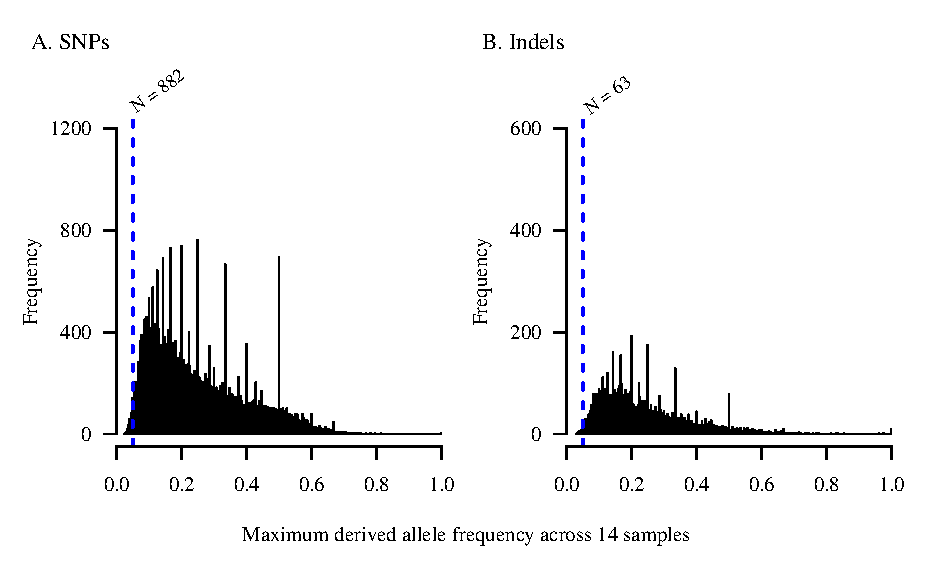
\includegraphics[width=1\textwidth]{Chp4_DNA/MAF_22.eps}
\caption[Distribution of the maximum derived (minor) allele frequency, $q$, for SNPs (A) and Indels (B).]{\textbf{Distribution of the maximum derived (minor) allele frequency, $q$, for SNPs (A) and Indels (B).} I expected alleles causing the observed fitness divergence between treatments to be segregating at moderately high frequency within at least one of the 14 pools. We, therefore, excluded from further consideration loci with a maximum minor allele frequency of 0.05 (dashed blue line represents $q = 0.05$; number of loci $q < 0.05$, $N$, labelled above the line). }
    \label{fig:FitmxMAF}
\end{figure}

\FloatBarrier

\begin{figure}[!h]
    \centering
    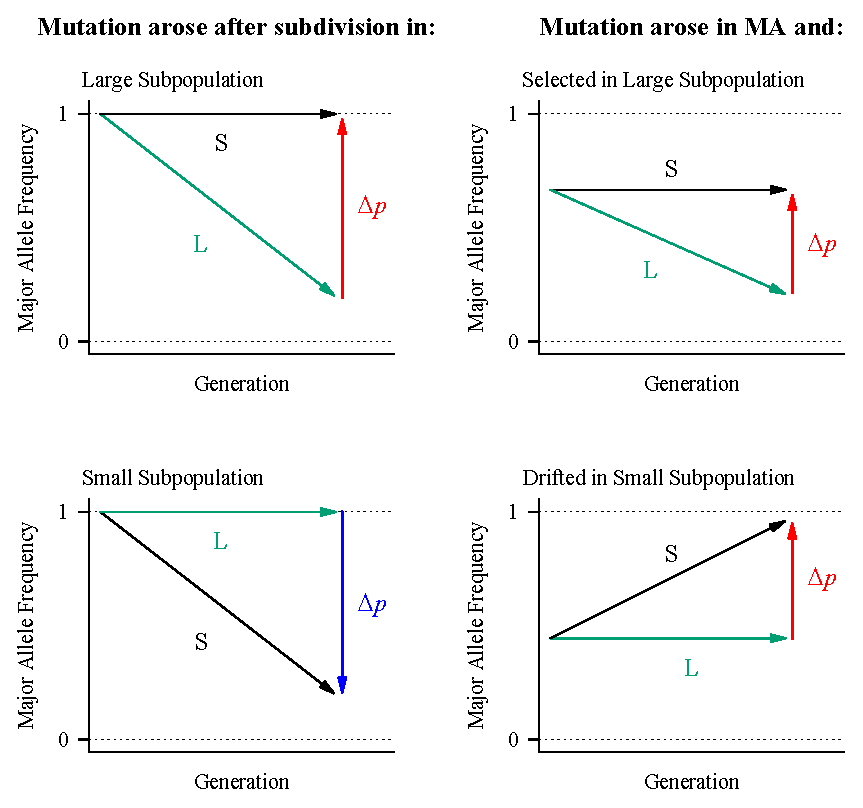
\includegraphics[width=0.75\textwidth]{Chp4_DNA/2023_predict_DeltaP_predict.eps}
\caption[Hypothetical scenarios for mutations contributing to high fitness and the corresponding trajectories of the focal allele frequencies in the two population size treatments. ]{\textbf{Hypothetical scenarios for mutations contributing to high fitness and the corresponding trajectories of the focal allele frequencies in the two population size treatments.} Panels represent different possible patterns of divergence in allele frequency between treatments, $\Delta p = p_L-p_S$, where $p_L > p_S$ (positive $\Delta p$, vector shown in blue, in bottom left) or where $p_L < p_S$ (negative $\Delta p$, vector shown in red, in top left and both right hand panels). Arrows indicate the direction and rate of allele frequency change in the S (black) and L (green) treatments. Left panels depict scenarios where a mutation arises after line subdivision, and right panels represent a mutation arising prior, during the mutation accumulation phase. Notably, random sampling (both drift and experimental sampling to estimate allele frequencies) will cause variation around the trajectories, impacting my ability to detect a difference in some loci. Horizontal dash line, at $p = 0$ and $p = 1$, is included as a reference point. }
    \label{fig:FitScenario}
\end{figure}

\FloatBarrier

\begin{figure}[!h]
    \hspace{4.25cm}
    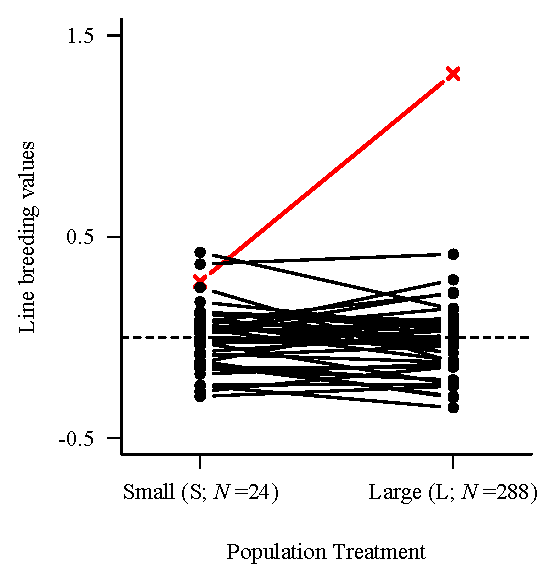
\includegraphics[width=0.45\textwidth]{Chp4_DNA/2023_Fit_blups.eps}
\caption[Breeding values for each of the forty-two mutation accumulation lines, within each of the population size treatments.]{\textbf{Breeding values for each of the forty-two mutation accumulation lines, within each of the population size treatments.} Breeding values were estimated as the best linear unbiased predictors (BLUPs) from Equation 1. Lines connect the BLUP estimate for the same MA line in each population size treatment. The Line 9 estimate (red cross) for the Large population size treatment is 6.0 SD above the mean.}
    \label{fig:FitBlups}
\end{figure}

\FloatBarrier

\begin{landscape}
\begin{figure}[!h]
    \centering
    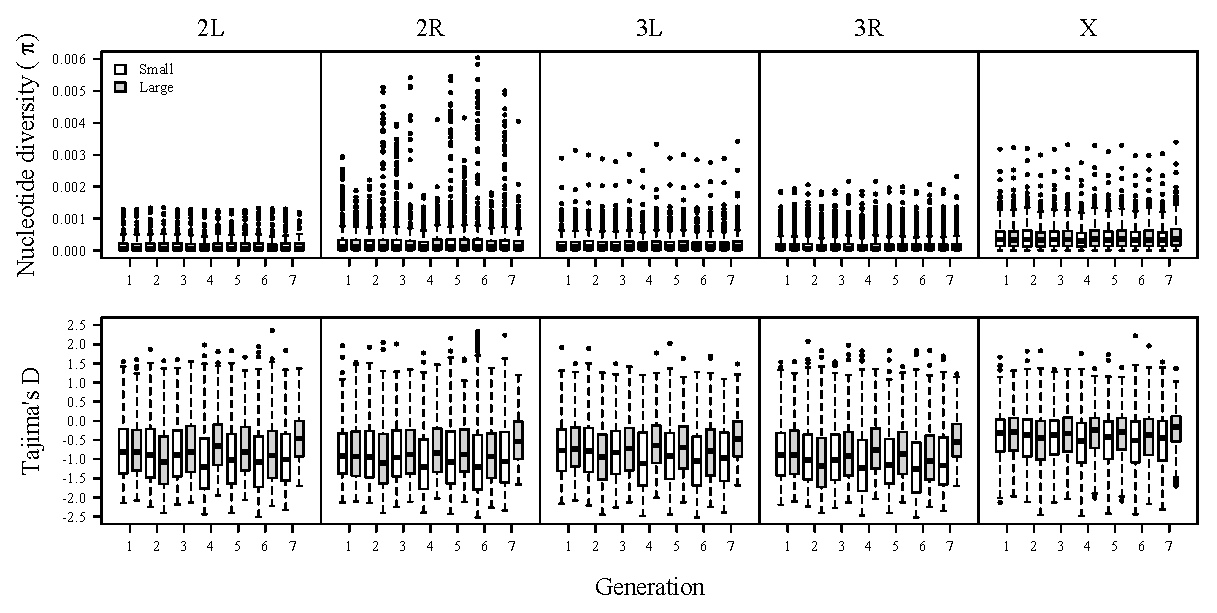
\includegraphics[width=1.2\textwidth]{Chp4_DNA/NucVsTajD.eps}
\caption[Distribution of genomic diversity estimates for 50 kbp non-overlapping windows for each of the \textit{D. serrata} pooled populations, for each of the chromosomal arms.]{\textbf{Distribution of genomic diversity estimates for 50 kbp non-overlapping windows for each of the \textit{D. serrata} pooled populations, for each of the chromosomal arms.} Each panel represents a chromosome arm (left to right), where the top row are nucleotide diversity ($\pi$) estimates and the bottom row are Tajima’s D. Treatments are shown separately (S treatment, white boxes; L treatment, grey boxes) for each of the seven generations (x-axis). Boxes represent the interquartile range (IQR), where black bars are the median; and whiskers are 1.5 times the IQR and dots represent estimates outside of this range. }
    \label{fig:FitNucDiv}
\end{figure}
\end{landscape}

\FloatBarrier

\begin{figure}[!h]
    \centering
    \includegraphics[width=0.85\textwidth]{Chp4_DNA/2023_FstNdeltapDists.pdf}
\caption[Distribution of the focal allele frequency differences ($\Delta p$) and pairwise $F_{ST}$ between the Large and the Small population treatment for the last two generations, estimated separately for SNPs and Indels.]{\textbf{Distribution of the focal allele frequency differences ($\Delta p$) and pairwise $F_{ST}$ between the Large and the Small population treatment for the last two generations, estimated separately for SNPs and Indels.} For each locus ($N= 98,189$), the focal [major] allele frequency of the S treatment was subtracted from the L treatment allele frequency ($\Delta p$) for the sixth (grey bars) and seventh (red bars) generation where the distributions are plotted separately for SNPs (A) and indels (C). Grey [red] vertical dashed lines represent the $2.5^{th}$ and $97.5^{th}$ percentiles for the distribution of $\Delta p$ in the sixth [seventh] generation. A total of 7963 unique SNPs (A: 4220, Gen 6 and 4192, Gen 7) and 1308 unique indels (C: 690, Gen 6 and 688, Gen 7) fell outside these tails. Again, for each locus, the pairwise $F_{ST}$ was estimated between treatments, for each generation (sixth: grey bars, seventh: red bars; SNPs: B; indels: D). The one-tailed $95^{th}$ percentile is represented by the grey [red] vertical dashed line for the sixth [seventh] generation, where 8409 SNPs (B: 4357, Gen 6 and 4451, Gen 7) and 1375 (D: 723, Gen 6 and 729, Gen 7) indels fell in this tail. (E, F) Venn diagrams represent the 12,352 unique outlier loci (E: 10,610 SNPs; and, F: 1,742 indels) identified across $\Delta p$ (two left ellipses) and $F_{ST}$ (two right ellipses) and in the sixth (grey) and seventh (red) generation. Numbers in overlapping ellipse regions represent the total of shared loci.}
    \label{fig:FitFstNdeltapDists}
\end{figure}

\FloatBarrier
\begin{figure}[!h]
    \centering
    \includegraphics[width=0.89\textwidth]{Chp4_DNA/2023_BarplotOutANN.pdf}
\caption[SnpEff annotated SNP and indel distribution for the outlier loci.]{\textbf{SnpEff annotated SNP and indel distribution for the outlier loci.} Plotted are the outliers (SNPs, $N= 208$; Indels, $N = 40$) identified by both methods ($\Delta p$ and $F_{ST}$), and in both terminal generations of the experiment (generation 6 and 7; see Venn diagrams in Figure \ref{fig:FitNucDiv}). Loci are binned by site class, determined by SnpEff annotation. SnpEff reports intragenic as variants within a gene but with no transcripts and are considered separate from intronic variants; however, I have included these within ‘intronic’ sites. Bars represent loci where there is positive (Spearman’s rank coefficient, $\rho\Delta p > 0$; SNPs, solid blue; Indels, striped blue) or negative ($\rho\Delta p < 0$; SNPs, solid red; Indels, striped red) monotonic change in the focal allele difference between the large and small population treatment over time. (A) All outlier loci (excluding three loci where $\rho\Delta p = 0$) and (B) only loci with a moderate or greater monotonic change are plotted ($|\rho\Delta p| \geq 0.5$). }
    \label{fig:FitSNPannoDist}
\end{figure}

\newpage
\FloatBarrier
\bigskip
\begin{figure}[!h]
    \centering
    \includegraphics[width=0.95\textwidth]{Chp4_DNA/2023_Gen1_LvsDiff_L_2.pdf}
\caption[Heatmap of treatment divergence over time for outlier loci relative to the initial frequency of the focal allele ($p$, x-axis) and the change in frequency of the focal allele (y-axis) in the L treatment.]{\textbf{Heatmap of treatment divergence over time for outlier loci relative to the initial frequency of the focal allele ($p$, x-axis) and the change in frequency of the focal allele (y-axis) in the L treatment.} Plotted are the 248 consistent outliers (same description as in Figure \ref{fig:FitSNPannoDist}). Temporal allele frequency differences for the L treatment were determined using the average allele frequency of the two terminal generations (6 and 7) minus the average allele frequency of the two initial generations (1 and 2). Outliers are further categorised by allele frequency divergence across treatments (Spearman’s rank coefficient, $\rho\Delta p$), ranging from 1 to -1 (dark blue to dark red). SNPs (left panel) and indels (right panel) are plotted separately. The five SNPs that had an estimated low to moderate functional impact on phenotype using SnpEff are circled in black and labelled (syn: synonymous variant, low effect; mis: missense variant, moderate effect).}
    \label{fig:FitHeatmapDeltap}
\end{figure}

\FloatBarrier

% \FloatBarrier
% \begin{figure}[!h]
%     \centering
%     % \includegraphics[width=0.89\textwidth]{Chp4_DNA/2023_FstNdeltapDists.eps}
% \caption[]{}
%     \label{fig:FitNucDiv}
% \end{figure}

% \FloatBarrier

% %%%% TABLES %%%%%%%%%%%%
\begin{table}[!htp]
\renewcommand{\arraystretch}{1.3}
\begin{center}
\caption[Mean nucleotide diversity ($\pi$) and Tajima’s D for the \textit{D. serrata} pooled populations.]{\textbf{Mean nucleotide diversity ($\pi$) and Tajima’s D for the \textit{D. serrata} pooled populations.}
Means ($\pm$ SE) for $\pi$ and Tajima’s D were obtained for each of the 14 pooled populations (two Treatments by seven Generations) from estimates of non-overlapping 50 kbp windows with $>60\%$ coverage after depth filtering and subsampling. The number of windows (Windows) and number of SNPs (SNPs) per pool are reported.}
\label{tab:FitNucDiv}
\begin{tabular}{cccrm{1.2em}lm{0.1em}rl}
\toprule
\textbf{Treatment}	& \textbf{Generation} & \textbf{Windows} & \multicolumn{1}{c}{\textbf{SNPs}} & \multicolumn{2}{c}{\bfseries{$\pi(10^{-4})$}} & & \multicolumn{2}{c}{\textbf{Tajima's D}}\\
\midrule						
S	&    1	& 2,746 &	96,725 &	2.55 & ($\pm$0.07) & &	-0.720 & ($\pm$0.014)\\
&	2 &	2,755    & 97,392	& 2.50	& ($\pm$0.07)	& & -0.759 &	($\pm$0.015)\\
&	3 &	2,744 	& 100,006	& 2.56	& ($\pm$0.07)	& & -0.775 &	($\pm$0.015)\\
&	4 &	2,714    & 98,208	& 2.22	& ($\pm$0.05)	& & -0.967 &	($\pm$0.017)\\
&	5 &	2,740 	& 108,508	& 2.65	& ($\pm$0.08)	& & -0.859 &	($\pm$0.016)\\
&	6 &	2,727 	& 111,251	& 2.62	& ($\pm$0.09)	& & -0.944 &	($\pm$0.018)\\
&	7 &	2,727 	& 103,585	& 2.56	& ($\pm$0.08)	& & -0.861 &	($\pm$0.016)\\[1.5ex]
L &	  1	&    2,746 &  91,054	& 2.48	& ($\pm$0.07)	& & -0.694 &	($\pm$0.014)\\
&	2 &	2,722 &	104,624 & 2.55  & ($\pm$0.08) & & -0.885 & ($\pm$0.016)\\
&	3 &	2,752 &	94,498 & 2.56	 & ($\pm$0.08)	& & -0.699 & ($\pm$0.014)\\
&	4 &	2,758 &	90,945 & 2.58	 & ($\pm$0.07)	& & -0.610 & ($\pm$0.013)\\
&	5 &	2,750 &	97,560 & 2.63	 & ($\pm$0.08)	& & -0.687 & ($\pm$0.014)\\
&	6 &	2,747 &	95,385 & 2.43	 & ($\pm$0.07)	& & -0.776 & ($\pm$0.015)\\
&	7 &	2,767 &	76,375 & 2.54	 & ($\pm$0.07)	& & -0.445 & ($\pm$0.011)\\
\bottomrule
\end{tabular}
\end{center}
\end{table}

\FloatBarrier
% Light gray:
\definecolor{Gray}{gray}{0.75}
% Light cyan:
\definecolor{LightCyan}{rgb}{0.68,0.8,0.85}
\begin{landscape}
\begin{table}[!htp]
\renewcommand{\arraystretch}{1.1}
\begin{center}
\caption[\textit{Drosophila serrata} gene annotation for 53 candidate outliers with \textit{Drosophila melanogaster} orthologs. ]{\textbf{\textit{Drosophila serrata} gene annotation for 53 candidate outliers with \textit{Drosophila melanogaster} orthologs.} Description for Chr., Scaffold, Position, Ref, the same as Table~\ref{tab:DNAsupp63Invaraint}. Variant alleles (Annotated Allele) are either the Focal allele [MA ancestral], defined as the major allele ($p$) in the first generation of the small population, or as the derived [Minor, $q$] allele (Allele Type). See main text for description of the metrics of allele differentiation (Spearman’s coefficient, $\rho\Delta p$; Generation 1 allele frequency for the Large treatment, Gen 1 Large $p$; Averaged terminal minus the averaged initial allele frequency for the Large treatment, Terminal – Initial Large $p$; Generation 6 treatment allele frequency difference, $\Delta p$; Generation 6 pairwise $F_{ST}$). Using SnpEff \citep{Cing12}, loci were annotated to the \textit{Drosophila serrata} reference genome (Region), where genes within $5kb$ are reported (\textit{D.~serrata} Gene ID) and gene descriptions were from NCBI. Orthologs from \textit{Drosophila melanogaster} (\textit{D. melanogaster} Gene ID, Uniprot code in brackets) were found using OrthoDB \citep{Kuzn22}. Alternating shaded rows (blue and grey) indicate groups of loci within $1Mb$ distance.} 
    \tiny
\label{tab:Fit53outliers}
\begin{tabular}{ccS[table-format=8.0]cccS[table-format=1.2]S[table-format=1.2]S[table-format=1.2]S[table-format=1.2]S[table-format=1.2]cccc}
\toprule
\textbf{Chr.} & \textbf{Scaffold} & \textbf{POS} & \textbf{REF} & \textbf{Annotated Allele} &
\multicolumn{1}{m{0.8cm}}{\centering \textbf{Allele \\ Type}} & \textbf{$\rho\Delta p$} & 
\multicolumn{1}{m{0.8cm}}{\centering \textbf{Gen 1 \\ Large $p$}} & 
\multicolumn{1}{m{0.9cm}}{\centering \textbf{Terminal- \\ Initial \\ Large $p$}} & \textbf{$\Delta p$} & \textbf{$F_{ST}$} & \textbf{Region} & 
\multicolumn{1}{m{1 cm}}{\centering \textbf{\textit{D. serrata}\\ Gene ID}} & 
\multicolumn{1}{m{4cm}}{\centering \textbf{\textit{D. serrata} \\Gene Description}} & 
\multicolumn{1}{m{3.5cm}}{\centering \textbf{\textit{D. melanogaster} \\ Gene Name (Uniprot)}}\\
\midrule
2L & ScA8VGg\_542; & 14058852 & C & T & Derived & 0.64 & 0.71 & 0.11 & 0.19 & 0.05 & Intronic & 110179928 & uncharacterized & CG14352 (Q9VQ27)\\
\rowcolor{LightCyan}
 \cellcolor{White}&\cellcolor{White} HRSCAF=776 & 15844684 & T & TAC & Focal & 0.80 & 1.00 & 0.00 & 0.21 & 0.12 & Intronic & 110179178 & uncharacterized & dcma (M9PCK0), Taf12L (M9PCK0)\\
 \rowcolor{LightCyan}
\cellcolor{White} & 	
\cellcolor{White} & 15934441 & C & T & Focal & -0.89 & 0.88 & -0.14 & -0.17 & 0.09 & Intronic & 110179178 & uncharacterized & dcma (M9PCK0), Taf12L (M9PCK0)\\
 &  & 17133398 & C & T & Derived & 0.61 & 0.85 & 0.12 & 0.13 & 0.04 & Intergenic & \makecell{110183421,\\ 110183422} & protein I'm not dead yet-like & CG7309 (Q7KTF1)\\
 &  &  &  &  &  &  &  &  &  &  &  & 110183432 & fibroblast growth factor receptor homolog 2 & dpr2 (Q59DZ4)\\
  \rowcolor{Gray}
\cellcolor{White} & 	
\cellcolor{White} & 19824618 & A & T & Focal & 0.50 & 0.53 & 0.15 & 0.21 & 0.05 & Intergenic & 110178131 & homeobox protein goosecoid & Gsc (A0A0S0WGV8)\\
  \rowcolor{Gray}
\cellcolor{White} & 	
\cellcolor{White} &  &  &  &  &  &  &  &  &  &  & 110178144 & homeobox protein aristaless & Pph13 (Q9XZU0)\\
   \rowcolor{Gray}
\cellcolor{White} & 	
\cellcolor{White} & 19824620 & G & A & Focal & 0.50 & 0.53 & 0.16 & 0.22 & 0.05 & Intergenic & 110178131 & homeobox protein goosecoid & Gsc (A0A0S0WGV8)\\
   \rowcolor{Gray}
\cellcolor{White} & 	
\cellcolor{White} &  &  &  &  &  &  &  &  &  &  & 110178144 & homeobox protein aristaless & Pph13 (Q9XZU0)\\
   \rowcolor{Gray}
\cellcolor{White} & 	
\cellcolor{White} & 19824622 & T & G & Focal & 0.50 & 0.51 & 0.16 & 0.23 & 0.05 & Intergenic & 110178131 & homeobox protein goosecoid & Gsc (A0A0S0WGV8)\\
   \rowcolor{Gray}
\cellcolor{White} & 	
\cellcolor{White} & &  &  &  &  &  &  &  &  &  & 110178144 & homeobox protein aristaless & Pph13 (Q9XZU0)\\
 \rowcolor{LightCyan}
\cellcolor{White} & 	
\cellcolor{White} ScA8VGg\_718; & 94346 & G & T & Focal & 0.71 & 0.79 & 0.10 & 0.14 & 0.03 & Intergenic & 110191704 & E3 SUMO-protein ligase PIAS2-like & Su(var)2-10 (A0A0B4JCQ7)\\
 \rowcolor{LightCyan}
\cellcolor{White} & 	
\cellcolor{White} HRSCAF=1046 & 94390 & A & T & Derived & 0.57 & 0.77 & 0.13 & 0.16 & 0.04 & Intergenic & 110191704 & E3 SUMO-protein ligase PIAS2-like & Su(var)2-10 (A0A0B4JCQ7)\\
 \midrule
 %%~~~~~~~~~~~~~~~~~~~~~~~~~~~~~~~~~~~~~~~~~~~~~~~~~~~~~%%
    \rowcolor{Gray}
\cellcolor{White}2R & \cellcolor{White}ScA8VGg\_785; & 2505651 & C & T & Derived & -0.68 & 0.97 & -0.15 & -0.16 & 0.07 & Intronic & 110177915 & protein grainyhead & grh (A0A0B4K7F6)\\
   \rowcolor{Gray}
\cellcolor{White} &\cellcolor{White} HRSCAF=1140 & 3355681 & A & AATATAT & Focal & 0.71 & 0.65 & 0.13 & 0.26 & 0.08 & Intronic & 110180256 & formin-J & CG13193 (A0A0B4K7X1),\\
   \rowcolor{Gray}
 \cellcolor{White}& \cellcolor{White} &  &  &  &  &  &  &  &  &  &  &  &  & ths (A0A0B4K7X1),\\
   \rowcolor{Gray}
 \cellcolor{White}& \cellcolor{White} &  &  &  &  &  &  &  &  &  &  &  &  & Ir48c (A1Z8P2), ths (A1Z8P2)\\
 &  & 13138985 & G & T & Focal & -0.57 & 0.56 & -0.11 & -0.17 & 0.03 & Intronic & 110185274 & F-actin-uncapping protein LRRC16A & LRR (A0A0B4KEE7)\\
 &  & 17148862 & C & CA & Focal & 0.71 & 0.78 & 0.14 & 0.19 & 0.08 & Intergenic & 110179690 & uncharacterized & CG13884 (Q8T974)\\
 &  &  &  &  &  &  &  &  &  &  &  & 110181281 & uncharacterized & CG30098 (Q4V653)\\
 &  & 27862559 & G & A & Focal & -0.50 & 0.48 & -0.11 & -0.18 & 0.03 & Intergenic & 110182853 & mitogen-activated protein kinase ERK-A & rl (A8Y4W5)\\
 &  &  &  &  &  &  &  &  &  &  &  & 110182855 & GRB10-interacting GYF protein 2-like & CG15877 (Q9W019)\\
 \midrule
  %%~~~~~~~~~~~~~~~~~~~~~~~~~~~~~~~~~~~~~~~~~~~~~~~~~~~~~%%
3L & ScA8VGg\_628; & 156715 & G & A & Derived & -0.50 & 0.62 & -0.10 & -0.20 & 0.04 & Intergenic & 110182513 & poly [ADP-ribose] polymerase-like & \\
 & HRSCAF=890 & 21124803 & T & G & Derived & -0.71 & 0.58 & -0.10 & -0.17 & 0.03 & Intronic & 110183674 & uncharacterized & Ack (Q9VZI2)\\
 &  &  &  &  &  &  &  &  &  &  &  & 110183695 & uncharacterized & CG7839 (Q8MSS0)\\
  \rowcolor{LightCyan}
 \cellcolor{White}& \cellcolor{White} & 22449044 & A & T & Derived & 0.64 & 0.59 & 0.11 & 0.20 & 0.04 & Intronic & 110178651 & unc-112-related protein & Fit1 (Q9VZI3), Fit2 (Q9VVD2)\\
   \rowcolor{LightCyan}
 \cellcolor{White}& \cellcolor{White} &  &  &  &  &  &  &  &  &  &  & 110178654 & putative mediator of RNA polymerase II  & anon-WO0140519.252 (E1JIC5),  \\
   \rowcolor{LightCyan}
 \cellcolor{White}& \cellcolor{White} &  &  &  &  &  &  &  &  &  &  &  & transcription subunit 26& CG14995-RC (E1JIC5),\\
   \rowcolor{LightCyan}
 \cellcolor{White}& \cellcolor{White} &  &  &  &  &  &  &  &  &  &  &  & & CT34848 (E1JIC5), NEST:bs15f01 (E1JIC5)\\
   \rowcolor{LightCyan}
 \cellcolor{White}& \cellcolor{White} & 22977069 & A & AAGG & Derived & -0.57 & 0.51 & -0.13 & -0.19 & 0.04 & Intronic & 110178615 & tryptophan 5-hydroxylase 1 & Trh (Q9W0K2)\\
   \rowcolor{LightCyan}
 \cellcolor{White}& \cellcolor{White} &  &  &  &  &  &  &  &  &  &  &  & uncharacterized & CG13912 (Q9W0K3)\\
 &  & 24866717 & T & A & Focal & -0.50 & 0.65 & -0.14 & -0.20 & 0.04 & Intergenic & 110188856 & uncharacterized & CG13810 (Q9W044)\\
 \rowcolor{Gray}
 \cellcolor{White}& \cellcolor{White}   & 30583524 & A & C & Derived & -0.54 & 0.70 & -0.11 & -0.17 & 0.03 & Intronic & 110178802 & uncharacterized & \\
 \rowcolor{Gray}
 \cellcolor{White}& \cellcolor{White}  & 30583527 & A & T & Derived & -0.54 & 0.72 & -0.12 & -0.19 & 0.04 & Intronic & 110178802 & uncharacterized & \\
  %%~~~~~~~~~~~~~~~~~~~Gap~~~~~~~~~~~~~~~~~~~~~~~~%%
 \bottomrule
\end{tabular}
\end{center}
\end{table}
\newpage
\begin{table}[!htp]
\renewcommand{\arraystretch}{1.1}
\begin{center}
    \tiny
\begin{tabular}{ccS[table-format=8.0]cccS[table-format=1.2]S[table-format=1.2]S[table-format=1.2]S[table-format=1.2]S[table-format=1.2]cccc}
\toprule
\textbf{Chr.} & \textbf{Scaffold} & \textbf{POS} & \textbf{REF} & \textbf{Annotated Allele} &
\multicolumn{1}{m{0.8cm}}{\centering \textbf{Allele \\ Type}} & \textbf{$\rho\Delta p$} & 
\multicolumn{1}{m{0.8cm}}{\centering \textbf{Gen 1 \\ Large $p$}} & 
\multicolumn{1}{m{0.9cm}}{\centering \textbf{Terminal- \\ Initial \\ Large $p$}} & \textbf{$\Delta p$} & \textbf{$F_{ST}$} & \textbf{Region} & 
\multicolumn{1}{m{1 cm}}{\centering \textbf{\textit{D. serrata}\\ Gene ID}} & 
\multicolumn{1}{m{4cm}}{\centering \textbf{\textit{D. serrata} \\Gene Description}} & 
\multicolumn{1}{m{3.5cm}}{\centering \textbf{\textit{D. melanogaster} \\ Gene Name (Uniprot)}}\\
\midrule
%%~~~~~~~~~~~~~~~~~~~Gap~~~~~~~~~~~~~~~~~~~~~~~~%%
3R & ScA8VGg\_76; & 2373892 & T & A & Derived & -0.50 & 0.83 & -0.11 & -0.15 & 0.03 & Intronic & 110186255 & protein lap4 & scrib (A0A0B4KHN3, A0A0B4K6I1)\\
 & HRSCAF=120  & 12282680 & T & A & Focal & 0.64 & 0.76 & 0.12 & 0.25 & 0.09 & Intergenic & 110176477 & cell differentiation protein RCD1 homolog & CG2053 (Q9V9S3)\\
    \rowcolor{LightCyan}
 \cellcolor{White}
 & \cellcolor{White} & 17882837 & C & T & Focal & 0.76 & 1.00 & 0.00 & 0.13 & 0.07 & Intronic & 110191392 & uncharacterized & side-III (Q0KIB0)\\
 \rowcolor{LightCyan}
 \cellcolor{White}
  & \cellcolor{White} & 17882838 & T & C & Focal & 0.76 & 1.00 & 0.00 & 0.13 & 0.07 & Intronic & 110191392 & uncharacterized & side-III (Q0KIB0)\\
 &  & 22464595 & T & TATAC & Focal & 0.57 & 0.87 & 0.10 & 0.15 & 0.05 & Intergenic & 110177159 & BTB/POZ domain-containing protein KCTD12 & Ktl (Q9VDH3)\\
 &  &  &  &  &  &  &  &  &  &  &  & 110177166 & glutamate receptor ionotropic, kainate 2 & KaiR1D (Q8MS48)\\
  \rowcolor{Gray}
 \cellcolor{White}
  & \cellcolor{White} & 34715464 & A & T & Derived & 0.64 & 0.67 & 0.12 & 0.16 & 0.03 & Intergenic & 110185346 & dynein light chain 1, cytoplasmic-like & \\
 \rowcolor{Gray}
 \cellcolor{White}
  & \cellcolor{White} &34715466 & G & T & Derived & 0.71 & 0.67 & 0.11 & 0.16 & 0.03 & Intergenic & 110185346 & dynein light chain 1, cytoplasmic-like & \\
 \rowcolor{LightCyan}
 \cellcolor{White}
  & \cellcolor{White} & 36020861 & T & G & Derived & 0.50 & 0.84 & 0.11 & 0.18 & 0.07 & Intergenic & 110180279 & acetylcholine receptor subunit alpha-like & \\
 \rowcolor{LightCyan}
 \cellcolor{White}
  & \cellcolor{White} & 36020862 & T & G & Derived & 0.50 & 0.84 & 0.11 & 0.18 & 0.07 & Intergenic & 110180279 & acetylcholine receptor subunit alpha-like & \\
 \rowcolor{LightCyan}
 \cellcolor{White}
  & \cellcolor{White} & 36020864 & T & G & Derived & 0.50 & 0.84 & 0.11 & 0.18 & 0.07 & Intergenic & 110180279 & acetylcholine receptor subunit alpha-like & \\
 \rowcolor{LightCyan}
 \cellcolor{White}
  & \cellcolor{White} & 36020867 & G & A & Derived & 0.50 & 0.85 & 0.11 & 0.18 & 0.07 & Intergenic & 110180279 & acetylcholine receptor subunit alpha-like & \\
 \rowcolor{LightCyan}
 \cellcolor{White}
  & \cellcolor{White} & 36020868 & A & T & Derived & 0.50 & 0.85 & 0.11 & 0.17 & 0.06 & Intergenic & 110180279 & acetylcholine receptor subunit alpha-like & \\
 &  & 37656500 & G & A & Derived & 0.71 & 0.53 & 0.12 & 0.19 & 0.04 & Intergenic & 110180482 & fatty acid synthase & FASN3 (Q7PLB8)\\
 &  &  &  &  &  &  &  &  &  &  &  & 110183954 & homeobox protein Nkx-2.1 & scro (A8Y525)\\
  \midrule
  %%~~~~~~~~~~~~~~~~~~~~~~~~~~~~~~~~~~~~~~~~~~~~~~~~~~~~~%%
  \rowcolor{Gray}
 \cellcolor{White}X & \cellcolor{White}ScA8VGg\_594; & 1192840 & C & A & Derived & 0.64 & 0.77 & 0.10 & 0.17 & 0.04 & Intronic & 110187043 & uncharacterized & gce (Q9VXW7)\\
   \rowcolor{Gray}
 \cellcolor{White}
 & \cellcolor{White} HRSCAF=845& 1719731 & T & TGTTGCAAGT - & Focal & 0.57 & 0.58 & 0.12 & 0.21 & 0.05 & Intronic & 110182462 & sex peptide receptor & SPR (A0A6H2EEN9)\\
   \rowcolor{Gray}
 \cellcolor{White}
 & \cellcolor{White} &  &  & AGCAAGTTGCTG &  &  &  &  &  &  &  &  & & \\[1ex]
 &  & 7843237 & A & AGGTAGGAAG & Focal & 0.76 & 1.00 & 0.00 & 0.14 & 0.08 & Intronic & 110180378 & integrin alpha-PS1 & mew (X2JDJ5)\\
 &  & 11361180 & T & C & Derived & 0.79 & 0.49 & 0.11 & 0.19 & 0.04 & Intronic & 110179504 & uncharacterized & m (Q9VYU8)\\
    \rowcolor{LightCyan}
  \cellcolor{White} & \cellcolor{White} & 12832334 &  C & T & Derived & -0.64 & 0.56 & -0.12 & -0.18 & 0.03 & Intergenic &  110181485  &  rho-associated protein kinase 2 & Rok (Q9VXE3)\\
    \rowcolor{LightCyan}
 \cellcolor{White} & \cellcolor{White} & &  &  &  &  &  &  &  &  &  & 110181588 & nucleolar and coiled-body phosphoprotein 1 & CG9782 (Q9VXE4)\\
    \rowcolor{LightCyan}
 \cellcolor{White} & \cellcolor{White} & 12832337 & A & G & Derived & -0.64 & 0.57 & -0.13 & -0.20 & 0.04 & Intergenic & 110181485 & rho-associated protein kinase 2 & Rok (Q9VXE3)\\
    \rowcolor{LightCyan}
 \cellcolor{White} & \cellcolor{White} & &  &  &  &  &  &  &  &  &  & 110181588 & nucleolar and coiled-body phosphoprotein 1 & CG9782 (Q9VXE4)\\
 &  & 16206998 & C & \makecell{CGGGGGAGC -\\ GCCAGGCA} & Focal & 0.64 & 0.69 & 0.12 & 0.18 & 0.04 & Intronic & 110182054 & ADP,ATP carrier protein & Ant2 (O62526)\\
 &  &  &  &  &  &  &  &  &  &  &  & 110182092 & ADP,ATP carrier protein & sesB (D1Z385)\\
 &  & 18673610 & C & CAAACCCAATAA & Focal & 0.80 & 1.00 & 0.00 & 0.14 & 0.08 & Intronic & 110184410 & uncharacterized LOC110184410 & CG12432 (E1JJN5), CG8557 (E1JJN5)\\
 &  & 19954637 & C & T & Focal & -0.57 & 0.83 & -0.15 & -0.17 & 0.03 & Intergenic & \makecell{110184404,\\ 110184469}  & allatostatin-A receptor & AstA-R1 (Q9U721)\\
   \rowcolor{Gray}
 \cellcolor{White} & \cellcolor{White} & 22876416 & G & A & Derived & -0.50 & 0.79 & -0.12 & -0.21 & 0.05 & Intergenic & 110179749 & uncharacterized & CG12065 (A0A6H2EDG9)\\
   \rowcolor{Gray}
 \cellcolor{White} & \cellcolor{White} & 23157828 & T & C & Derived & 0.50 & 0.80 & 0.10 & 0.16 & 0.05 & Intergenic & 110179751 & irregular chiasm C-roughest protein & rst (Q08180)\\
   \rowcolor{Gray}
 \cellcolor{White} & \cellcolor{White} & 23157832 & G & A & Derived & 0.50 & 0.78 & 0.11 & 0.17 & 0.06 & Intergenic & 110179751 & irregular chiasm C-roughest protein & rst (Q08180)\\
   \rowcolor{Gray}
 \cellcolor{White} &  \cellcolor{White} & 23157836 & T & C & Derived & 0.50 & 0.78 & 0.11 & 0.18 & 0.06 & Intergenic & 110179751 & irregular chiasm C-roughest protein & rst (Q08180)\\
    \rowcolor{LightCyan}
 \cellcolor{White} & \cellcolor{White} & 24638156 & G & T & Focal & -0.71 & 0.76 & -0.10 & -0.18 & 0.04 & Intergenic & 110184546 & uncharacterized & Ir7e (B7Z0X5)\\
    \rowcolor{LightCyan}
 \cellcolor{White} & \cellcolor{White}  & &  &  &  &  &  &  &  &  &  & 110184569 & uncharacterized & Ir7g (Q9W3P0)\\
    \rowcolor{LightCyan}
 \cellcolor{White} & \cellcolor{White} & &  &  &  &  &  &  &  &  &  & 110184571 & uncharacterized & Ir7f (B7Z0X6)\\
    \rowcolor{LightCyan}
 \cellcolor{White} & \cellcolor{White} & 24763012 & C & T & Focal & -0.71 & 0.73 & -0.11 & -0.19 & 0.04 & Intronic & 110184530 & protein tweety & tty (M9PFD6)\\
   \rowcolor{Gray}
 \cellcolor{White}
 & \cellcolor{White}  & 26698570 & T & A & Derived & 0.71 & 0.63 & 0.11 & 0.16 & 0.03 & Intergenic & 110175994 & uncharacterized & r-cup (Q9VRD3)\\
   \rowcolor{Gray}
 \cellcolor{White}
 & \cellcolor{White}  & 27015057 & C & T & Derived & 0.57 & 0.61 & 0.12 & 0.22 & 0.05 & Intergenic & 110175950 & transcriptional regulator ATRX homolog & CG1324 (Q9VRB7)\\
   \rowcolor{Gray}
 \cellcolor{White}
 & \cellcolor{White} & 27919844 & A & ATTC & Focal & 0.76 & 1.00 & 0.00 & 0.18 & 0.10 & Intergenic & 110175943 & pickpocket protein 28 & ppk8 (B7Z123)\\
    \rowcolor{Gray}
 \cellcolor{White}
 & \cellcolor{White}  &  &  &  &  &  &  &  &  &  &  & 110176018 & uncharacterized & CG32547 (A1KXD5)\\
 &  & 29444741 & \makecell{TTGTAC -\\TTGTTTC} & \makecell{CTGTACTTGTTTC \\(T)} & \makecell{Focal\\(Derived)} & 0.64 & 0.81 & 0.12 & 0.17 & 0.05 & Intronic & 110180283 & palmitoyltransferase app & \makecell{Zdhhc8 (A8JUM2),\\ CG12136 (M9NGX0)}\\

\bottomrule
\end{tabular}
\end{center}
\end{table}
\end{landscape}


% \begin{tabular}{ccS[table-format=8.0]ccccccS[table-format=2.0]S[table-format=1.2]S[table-format=1.3]}
% \toprule
% \textbf{Chr.} & \textbf{Scaffold} &
% \textbf{Position} & 
% \multicolumn{1}{m{0.8cm}}{\centering \textbf{Reference\\Allele}} &
% \multicolumn{1}{m{1.7cm}}{\centering \textbf{Focal Allele\\(major, $p$)}} &
% \multicolumn{1}{m{1.2cm}}{\centering \textbf{Minor Allele\\(minor, $q$)}} & 
% \textbf{Type} & \textbf{Region} &
% \multicolumn{1}{m{0.5cm}}{\centering \textbf{Max.\\MAF}} &
% \multicolumn{1}{m{1.1cm}}{\centering \textbf{Maximum\\minor allele\\coverage}} &
% \multicolumn{1}{m{1.1cm}}{\centering \textbf{Spearman's\\rank\\coefficient}} &
% \multicolumn{1}{m{1.2cm}}{\centering \textbf{Generation 6  \\ $F_{ST}$}}\\
\FloatBarrier